%!TEX TS-program = pdflatex
%!TEX root = main.tex
%!TEX encoding = UTF-8 Unicode


\section{GAN}
Uno tra i primi metodi che permettevano di generare immagini sintetiche faceva uso di una particolare versione di \emph{Auto-Encoder} i \emph{Variational Auto-Encoder}.
Come nel caso degli AE classici, i VAE hanno una struttura che ricorda una clessidra: la prima metà della rete permette di comprimere l'input, mappandolo in quello che viene chiamato spazio latente, di minor dimensione rispetto allo spazio di partenza;  la seconda metà, invece, prende l'input compresso e lo mappa nello spazio di partenza.
Durante il training si vuole ottimizzare la compressione in modo che non ci sia perdita di informazione, questo viene effettuato andando a minimizzare la distanza tra input originale ed input ricostruito.
Nei VAE, in corrispondenza del punto della rete in cui si raggiunge il livello massimo di compressione (\emph{bottleneck}), invece di essere generato il vettore compresso $z$, viene prodotta una coppia di vettori $\sigma$ e $\mu$ che descrivono una distribuzione di probabilità dei vettori compressi.
In questo modo è possibile campionare $z$ dalla distribuzione appena prima della decompressione.
Il campionamento non è un'operazione differenziabile e questo rende inapplicabile l'algoritmo della $backpropagation$, quindi risulta necessario effettuare quello che viene chiamato \emph{reparametrization trick}.
Rappresentando $z$ come $z = \mu + \sigma \odot \varepsilon$ in cui $\varepsilon \sim \mathcal{N}(0,1)$, quindi $\varepsilon$ è campionata da una distribuzione normale, è possible effettuare l'operazione di \emph{sampling} all'esterno della rete.
In questo modo $\mu$ e $\sigma$ possono essere utilizzati per il calcolo del gradiente e quindi usati durante la \emph{backpropagation}.

Dopo questa breve panoramica sulle VAE, ispirata alla lezione del MIT \cite{MIT_GEN}, ci si accorge che sono una soluzione astuta ma complessa e che le loro prestazioni sono vincolate strettamente allo spazio latente che si è trovato durante il training.
%TODO nota sul Disentanglement delle variabili che permette di avere controllo sulle singole caratteristiche delle immagini generate

Le \emph{Generative Adversarial Network} (GAN) sono state modellate appositamente per trovare un'altra soluzione al problema della creazione di immagini sintetiche.
Nelle GAN sono presenti due modelli che, citando \cite{GANTF}, \emph{``vengono addestrati simultaneamente da un processo contraddittorio. Un generatore ("l'artista") impara a creare immagini che sembrano reali, mentre un discriminatore ("il critico d'arte") impara a distinguere le immagini reali dai falsi''}.
Riformulando la frase si può dire che una GAN, come si vede in \autoref{fig:gan}, è composta da due reti: la prima viene chiamata Generatore $G$ ed il suo scopo è fornire in output un $x_{fake}$ che sembri appartenere alla distribuzione del \emph{dataset} reale fornito; la seconda, detta Discriminatore $D$, prende in input un $x_{fake}$ ed un $x_{real}$ estratto dal \emph{dataset} e deve riuscire a distinguere il dato reale da quello sintetico.
Quindi il training viene svolto in quattro momenti:
\begin{itemize}
  \item all'inizio $G$ a partire da del rumore randomizzo genera, basandosi sulle sue conoscenze attuali, un $x_{fake}$;
  \item successivamente $D$ stabilisce quale tra $x_fake$ ed un $x_real$ fornito è sintetico;
  \item la prestazione di $D$ viene valutata con il \emph{ground truth} e con questa può essere effettuata la \emph{backpropagation} su $D$;
  \item con l'output del discriminatore è possibile determinare anche la prestazione di $G$, infatti se questo è riuscito a confondere $D$ significa che sta raggiungendo una buona conoscenza del dominio.
\end{itemize}
Notare come $G$ sia in grado di mappare del rumore casuale nello spazio delle \emph{feature} del dominio e che quindi, una volta allenato, possa essere sfruttato molto facilmente: basterà avere del rumore da cui partire.
\begin{figure}[ht]
  \centering
  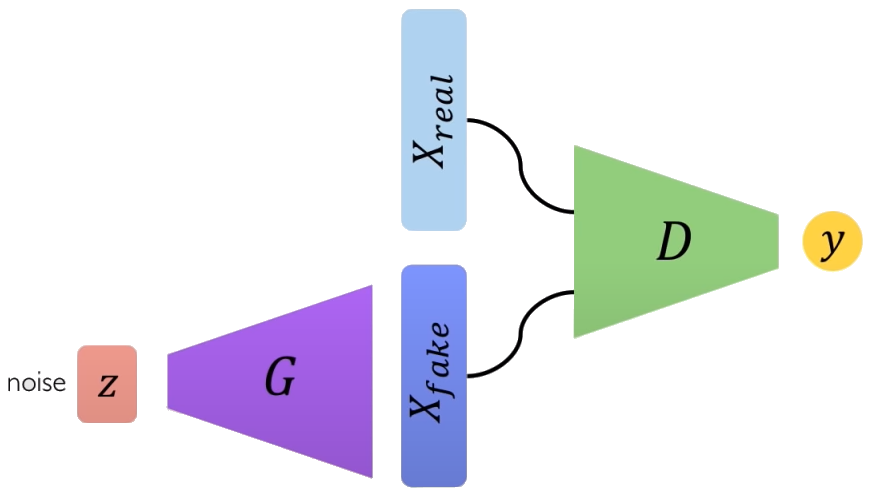
\includegraphics[width=.7\textwidth]{GAN/arch.png}
  \caption{Architettura di una generica GAN (dalle slide in \cite{MIT_GEN})}
  \label{fig:gan}
\end{figure}
Rispetto ai $VAE$ le $GAN$ risultano non solo più intuitive ma permettono anche di raggiungere prestazioni veramente sorprendendo, come si può vedere il \cit{GAN_HD}, in cui anche gli esperti umani hanno 




% L'efficacia di questa tecnica e' lampante quando si parla di immagini...
%In questo caso si fa riferimento alla possibilità di utilizzare le GAN come generatori di immagini sintetiche indistinguibili da quelle reali, in \cite{GAN_HD} si può osservare il livello di dettaglio impressionante che queste reti sono in grado di produrre.



